\documentclass{article}
\usepackage[utf8]{inputenc}
\usepackage{amsmath}
\usepackage{amsfonts}
\usepackage[]{graphicx}
\usepackage[legalpaper, portrait, margin = 1in]{geometry}
\usepackage{amsmath}
\usepackage{amssymb}
\usepackage{amsthm}
\usepackage[utf8]{inputenc}
\usepackage{amsmath}
\usepackage{amsfonts}
\usepackage[]{graphicx}
\usepackage[a4paper, portrait, margin = 1in]{geometry}
\usepackage{enumitem}
\usepackage{xcolor}

%darkmode
%\pagecolor[rgb]{0.2,0.19,0.18} 
%\color[rgb]{0.92,0.86,0.7}

\newenvironment*{alphenum}{\begin{enumerate}[label= (\alph*)]}{\end{enumerate}}

\graphicspath{{./images/}}

\begin{document}
\Huge 

Math 211 Quick reference

\normalsize

\section{Vectors}

\begin{df}
The formula for projection is as follows:
\[proj_{\overrightarrow{v}} \overrightarrow{u} = \frac{\overrightarrow{u}\cdot\overrightarrow{v}}
{\|\overrightarrow{u}\|}\overrightarrow{u}\]
\end{df}

\begin{df}
To find the cross product of two vectors $\overrightarrow{u}$ and $\overrightarrow{b}$
, we take the determinant of the matrix: 

\[
\overrightarrow{u} \times \overrightarrow{v}=   
\begin{vmatrix}
i & j & k \\
u_1 & u_2 & u_3 \\
v_1 & v_2 & v_3
\end{vmatrix}\]
\par Where i, j, k are columns of the identity matrix $I_3$.

This gives us a vector of the form

\[ 
\overrightarrow{u} \times \overrightarrow{v}=   
\begin{bmatrix}    
\begin{vmatrix}
    u_2 & u_3\\
    v_2 & v_3
\end{vmatrix}, & 
-\begin{vmatrix}
    u_1 & u_3\\
    v_1 & v_3
\end{vmatrix}, &
\begin{vmatrix}
    u_1 & u_2\\
    v_1 & v_2
\end{vmatrix}
\end{bmatrix}   ^T 
\]
\end{df}

\section{Linear Transformations}
As far as this cheat sheet goes, the most important parts of this unit
will be the matrices of tranformation for simple transfomations such as 
reflections in a line with slope m, or rotations by $\theta$.

\par 

\begin{df}

First, the matrix of rotation (counterclockwise by $\theta$)
\[
\begin{bmatrix}
   \cos{\theta} & \sin{\theta}\\
   -\sin{\theta} & \cos{\theta}
\end{bmatrix}
\]
\end{df}
\begin{df}
Next, the matrix of reflection in a line with slope $m$:
\[
\frac{1}{m^2+1}
\begin{bmatrix}
    1-m^2 & 2m\\
    2m & m^2-1
\end{bmatrix}
\]
\end{df}
\begin{df}
Finally, the matrix of projection onto the line $y=mx$ is:
\[
\frac{1}{m^2+1}   
\begin{bmatrix}
    1 & m\\
    m & m^2
\end{bmatrix}
\]
\end{df}
\section{Complex Numbers}
Complex numbers have fewer formulas than other units, so rather than provide 
any formulas (there are few), I'm including methods to convert between forms
they can take, as well as procedures for different operations that can be 
taken on them\par 
First, we note that the standard form for complex numbers is $a+ib$
We denote this number $z$, $z \in \mathbb{C}$, and $a,b \in \mathbb{R}$.
Complex numbers in this form can be visualised on a cartesian plane,
with the real component $a$ plotted on the x-axis, and the 
complex component $b$ on the y-axis.
\newpage
\par 
Complex numbers can be imagined in a similar way on a cartesian plane,
however if we consider polar form, our variables change from 
$a,b$ to $\theta,r$.
\par
We can define these two variables using $a,b$ though. 
\[r = \sqrt[]{a^2+b^2}\]
\[\cos{\theta} = \frac{a}{r}\]
\[\sin{\theta} = \frac{b}{r}\]
Think of r as a scalar multiple, the length of the vector
from the origin to a,b. Then consider $\theta$ to be the 
angle between the x-axis and said vector.
\par 
Given all this, we have two ways to write $z$ in terms of 
$r$ and $\theta$. 
\[z = r e^{i \theta}\]
\[z = r(\cos{\theta}+i\sin{\theta})\]
Finally, it's important to note that 
\[r\cos{\theta} = a\]
\[ri\sin{\theta}= bi\]
\begin{center}
Because of the numerous references I've already had to make to my unit
circle, I'm including one here.\par 
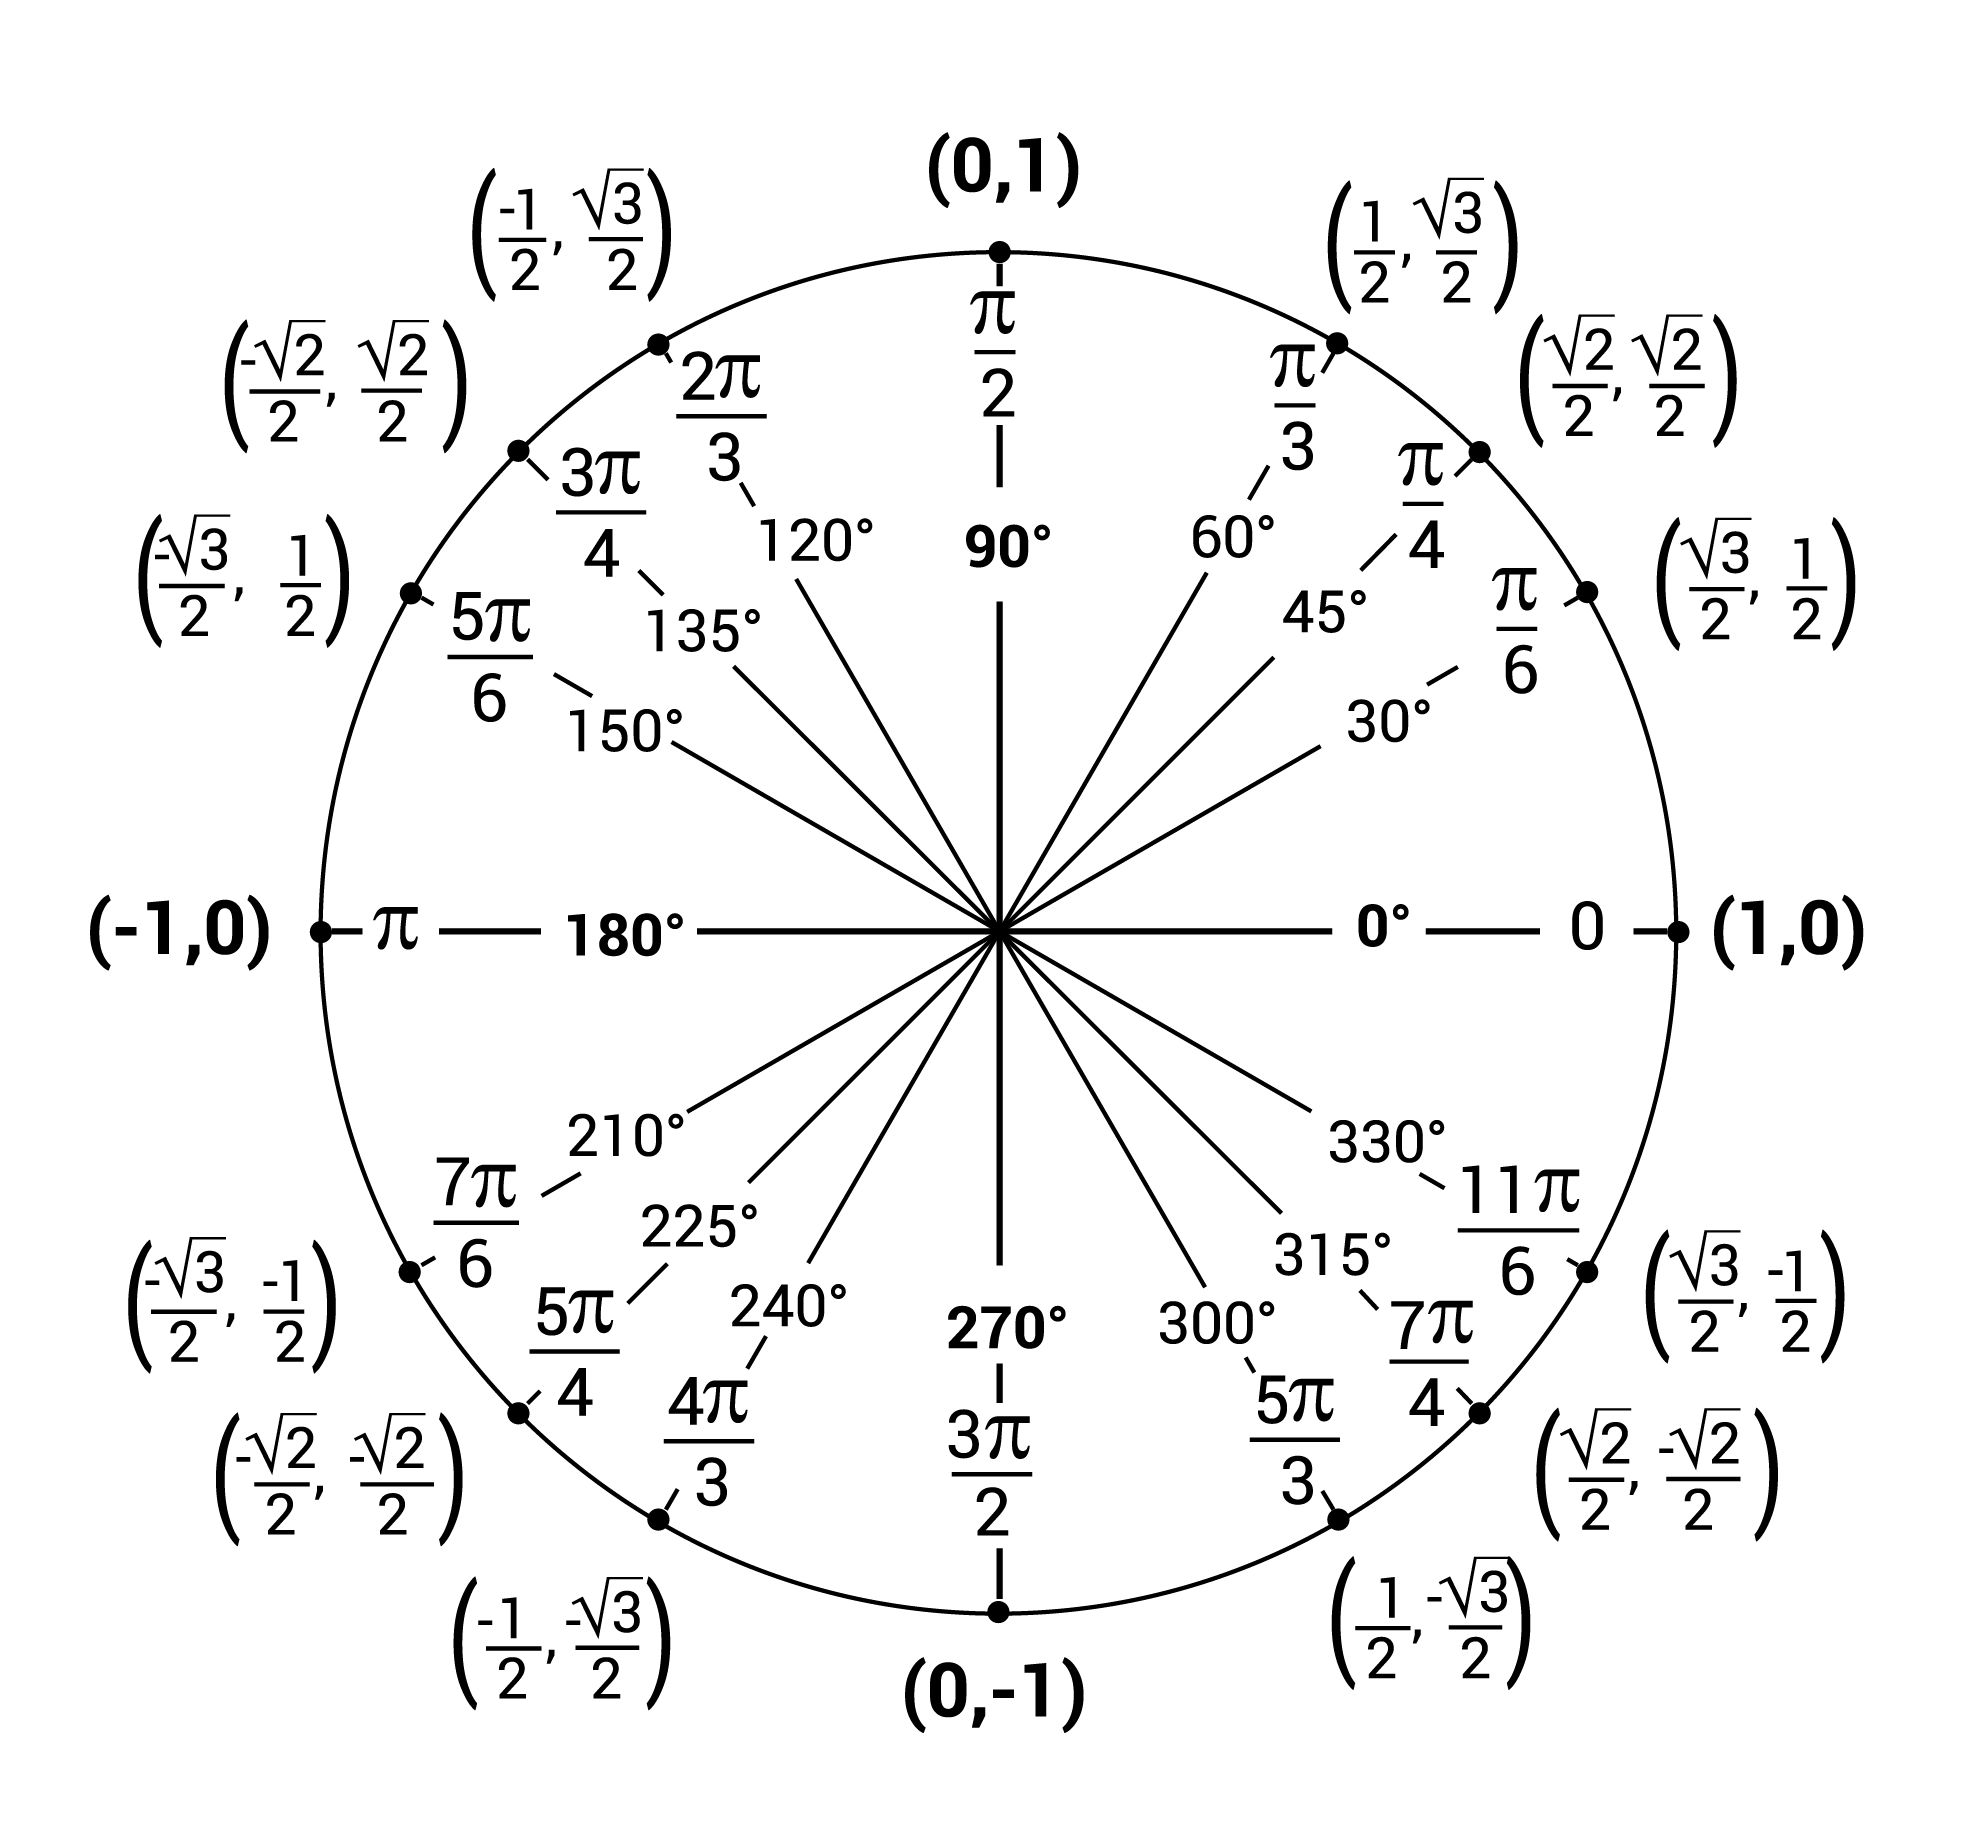
\includegraphics[scale=0.125]{Unit-circle}
\end{center}
De Moivre's theorem is critical to this unit for finding roots of complex numbers.
It is stated as follows:

\[{(e^{i\theta})}^n = e^{in\theta}\]

When we take the $k^{th}$ root of $z$, there are always 
k roots.
These roots can be found through the following process: \par  
Say we have a known complex number $w$ and an unknown root of $w$, $z$.
\[z^k = w\]
\[w=se^{i\phi}\]
\[z=re^{i\theta}\]
\[r^k e^{ik\theta}=se^{i\phi}\]
Using this, we can write in general that:
\[r^k=s\]
\newpage
However, we cannot write that ${ik\theta}={i\phi}$. Since there
must be k roots, we write that
\[n\theta = \phi+2\pi l\]
\begin{center}
For $l = 0,1,2,\dotsb,n-1$.
\end{center}
To provide full solutions for roots like these, we combine our values $\theta, r$ with our
polar form for $z$.
\par 

\par 
The quadratic equation can be used to find complex roots of some polyonomials.
Simply use the the equation how you normally would. However, where you would have 
claimed there were no solutions in Math 20, you can now take the negative root and
present the solution in the form of $a+bi$.
In some cases, the value b will be imaginary or complex. Simply proceed as normal,
the solution should simplify to a single complex number.
\par 
Here's the formula, for reference:
\[\frac{-b\pm \sqrt[]{b^2-4ac}}{2a}\]
\section{Spectral Theory}
An \textbf{Eigenvalue} is a value $\lambda$ such that a $n\times n$ matrix 
multiplied by a vector $X$ is equal to $\lambda X$. An \textbf{Eigenvector} 
in this case, would be $X$.
\par To find eigenvalues of a matrix A, we solve the equation for the \textbf{characteristic polynomial}:
\[det(xI-A)=0\]
\par To find the eigenvectors after we've found a $\lambda$, we can use the same 
equation, with the eigenvector X unknown.
\[(\lambda I - A)X=0\]
\par Of course, a zero vector would multiply with any matrix to equal itself, but we consider this to be a trivial solution, not a
true eigenvector. However, we can have an eigenvalue of 0, with the eigenvector being nonzero.
\par 
Similar matrices $A$ and $B$ are matrices such that a third invertible matrix
$P$ exists and:
\[A=P D P^{-1}\]
Assuming D is diagonal, it will be a matrix of size $n\times n$, where the only
entries are the eigenvalues of $A$ on the main diagonal.

For each eigenvalue $\lambda_n$ in $D$, a column $v_1$ in $P$ will be the eigenvector
corresponding to $\lambda_n$.\newline
\newline
\huge
Applications of Spectral Theory
\newline
\normalsize

One common application of spectral theory is in statistics. A \textbf{Markov Matrix}
is one where the sum of the values on every column is equal to 1. 
Markov matrices can be used to represent the chance of differentchanges between a list of states.
They can represent weather, population changes, and more.
\begin{ex}
    Consider a fox who lives in a forest with three regions, A, B, and C.
    The fox follows the following rules day-by-day.
    \begin{itemize}
        \item The fox will never hunt in the same region twice in a row.
        \item The fox will always hunt in C after A.
        \item After hunting in B or C, the fox is twice as likely to pick A opposed to the other choice.
    \end{itemize}
    What is the Markov Matrix for these criteria?
\end{ex}

After we have found a Markov Matrix, we can use it to determine the long-term 
state of an environment. We can find this using the formula $A-I=0$.
This gives us a vector with a parameter, and we choose the parameter such that the
entries of the vector sum to 1.

\par


\end{document}